\chapter{Phone Hardwares and Technologies}

As phones are much smaller than other gaming systems, it creates a limit to how powerful the components can be. The newest generation of smartphones does however have either quad cores or dual cores and support for OpenGL 2 Rendering and some also have HD screens which is some of the recommended specs for a phone used for gaming.

Some phones, and especially smartphones, does also have a bunch of hardware that most gaming systems does not have. Some of these hardwares include GPS, GyroMeter, Internet access everywhere as long there is service, and a battery that can provide power for an extended amount of time even when used for longer periods in a row.

In this chapter we will see how some of these hardwares may be used in a variety of ways, and possible ways of using them in a IRLVRMMO.


\section{GPS}

Global Positioning System (GPS) is used to track your location and can even be used to navigate a user between multiple points\cite{GPS}. Some modern GPS is even able to communicate with each other to warn against, for instance traffic jams. The possibility to communicate with each other and know each others locations in cooperative games is vital for players that want to work together as a team. A GPS is a vital component for a IRLVRMMO as it should be possible to have players placed in the world just as a character in a video game. Some sort of GPS or Coordinates are often also used in video games to locate players, and areas for the players to explore, which validates that a GPS for a IRLVRMMO will be necessary.

A common problem seen with GPS is that there is no signal to the satellites which then makes it hard to determine an exact location. There are other methods such as triangulation, and location determination through Wi-Fi, but these technologies is not as exact as GPS and it is mainly indoors or in extreme urban areas that the GPS signal may fail.


\section{Gyrometer}

The gyrometer is a hardware that some barely know exist, and what it can do, but it is used a lot for compass apps and Electro Magnetic Fields (EMF) meter. You can compare a gyrometer to a 3D axis where the gyrometer will offer a vector pointing a certain way depending on the rotation\cite{GyroMeter}. When we can use 3D vectors our possibilities is close to unlimited. In some shooting games they use ray cast, or trace lines, which simply is a line in some direction, in some length. You can translate a 3D vector into such ray cast and thereby possibly mimic First, or third person shooter games in the real world.


\section{Accessories}
\label{cha:Accessories}
There is ton of different accessories for phones that can be used in games. Some of them is stands where you can plug your phone into a holder and then have it mounted on a, for instance, toy gun that can tap the screen when you click the triggers on the gun\cite{LaserTag}. Similar guns with infra red transmitter and receiver have been used in laser tag games for phones as seen in\figref{fig:LaserTag}. With such accessories there are great possibilities to make a game feel real, but the question is whether such gun is legal to run around with on open streets, as they could be mistaken for actual weapons or paint ball guns.

\begin{figure}[H]
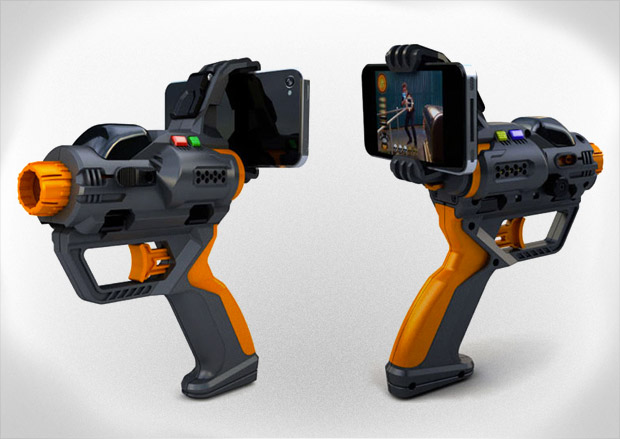
\includegraphics[width=0.5\linewidth]{img/LaserTag}
\centering
\caption{An image showing the laser tag toy guns for a laser tag game}
\label{fig:LaserTag}
\end{figure}